%% !TEX root =  paper.tex
\section{Approach}\label{sec:approach}

The goal of our approach is to find potential fixes that can repair a broken web test that was used to work correctly on a version $V$ of the AUT, and that now breaks when applied on a subsequent version $V+n$ (with usually $n=1$).

The focus of our technique is to repair \textit{locators}, that represent the main source of breakage.
Our technique can detect and correct locator problems that pertain to the breakage scenarios described in \autoref{sec:breakage-scenarios}.
Therefore, our approach analyses the execution of each statement,  asserts on its correctness through a visual ``inspection'' of the GUI, warns the developer of potential inconsistencies or breakages, and creates potential candidate repairs that fix them.

\begin{figure}[t]
\centering
%\fbox{
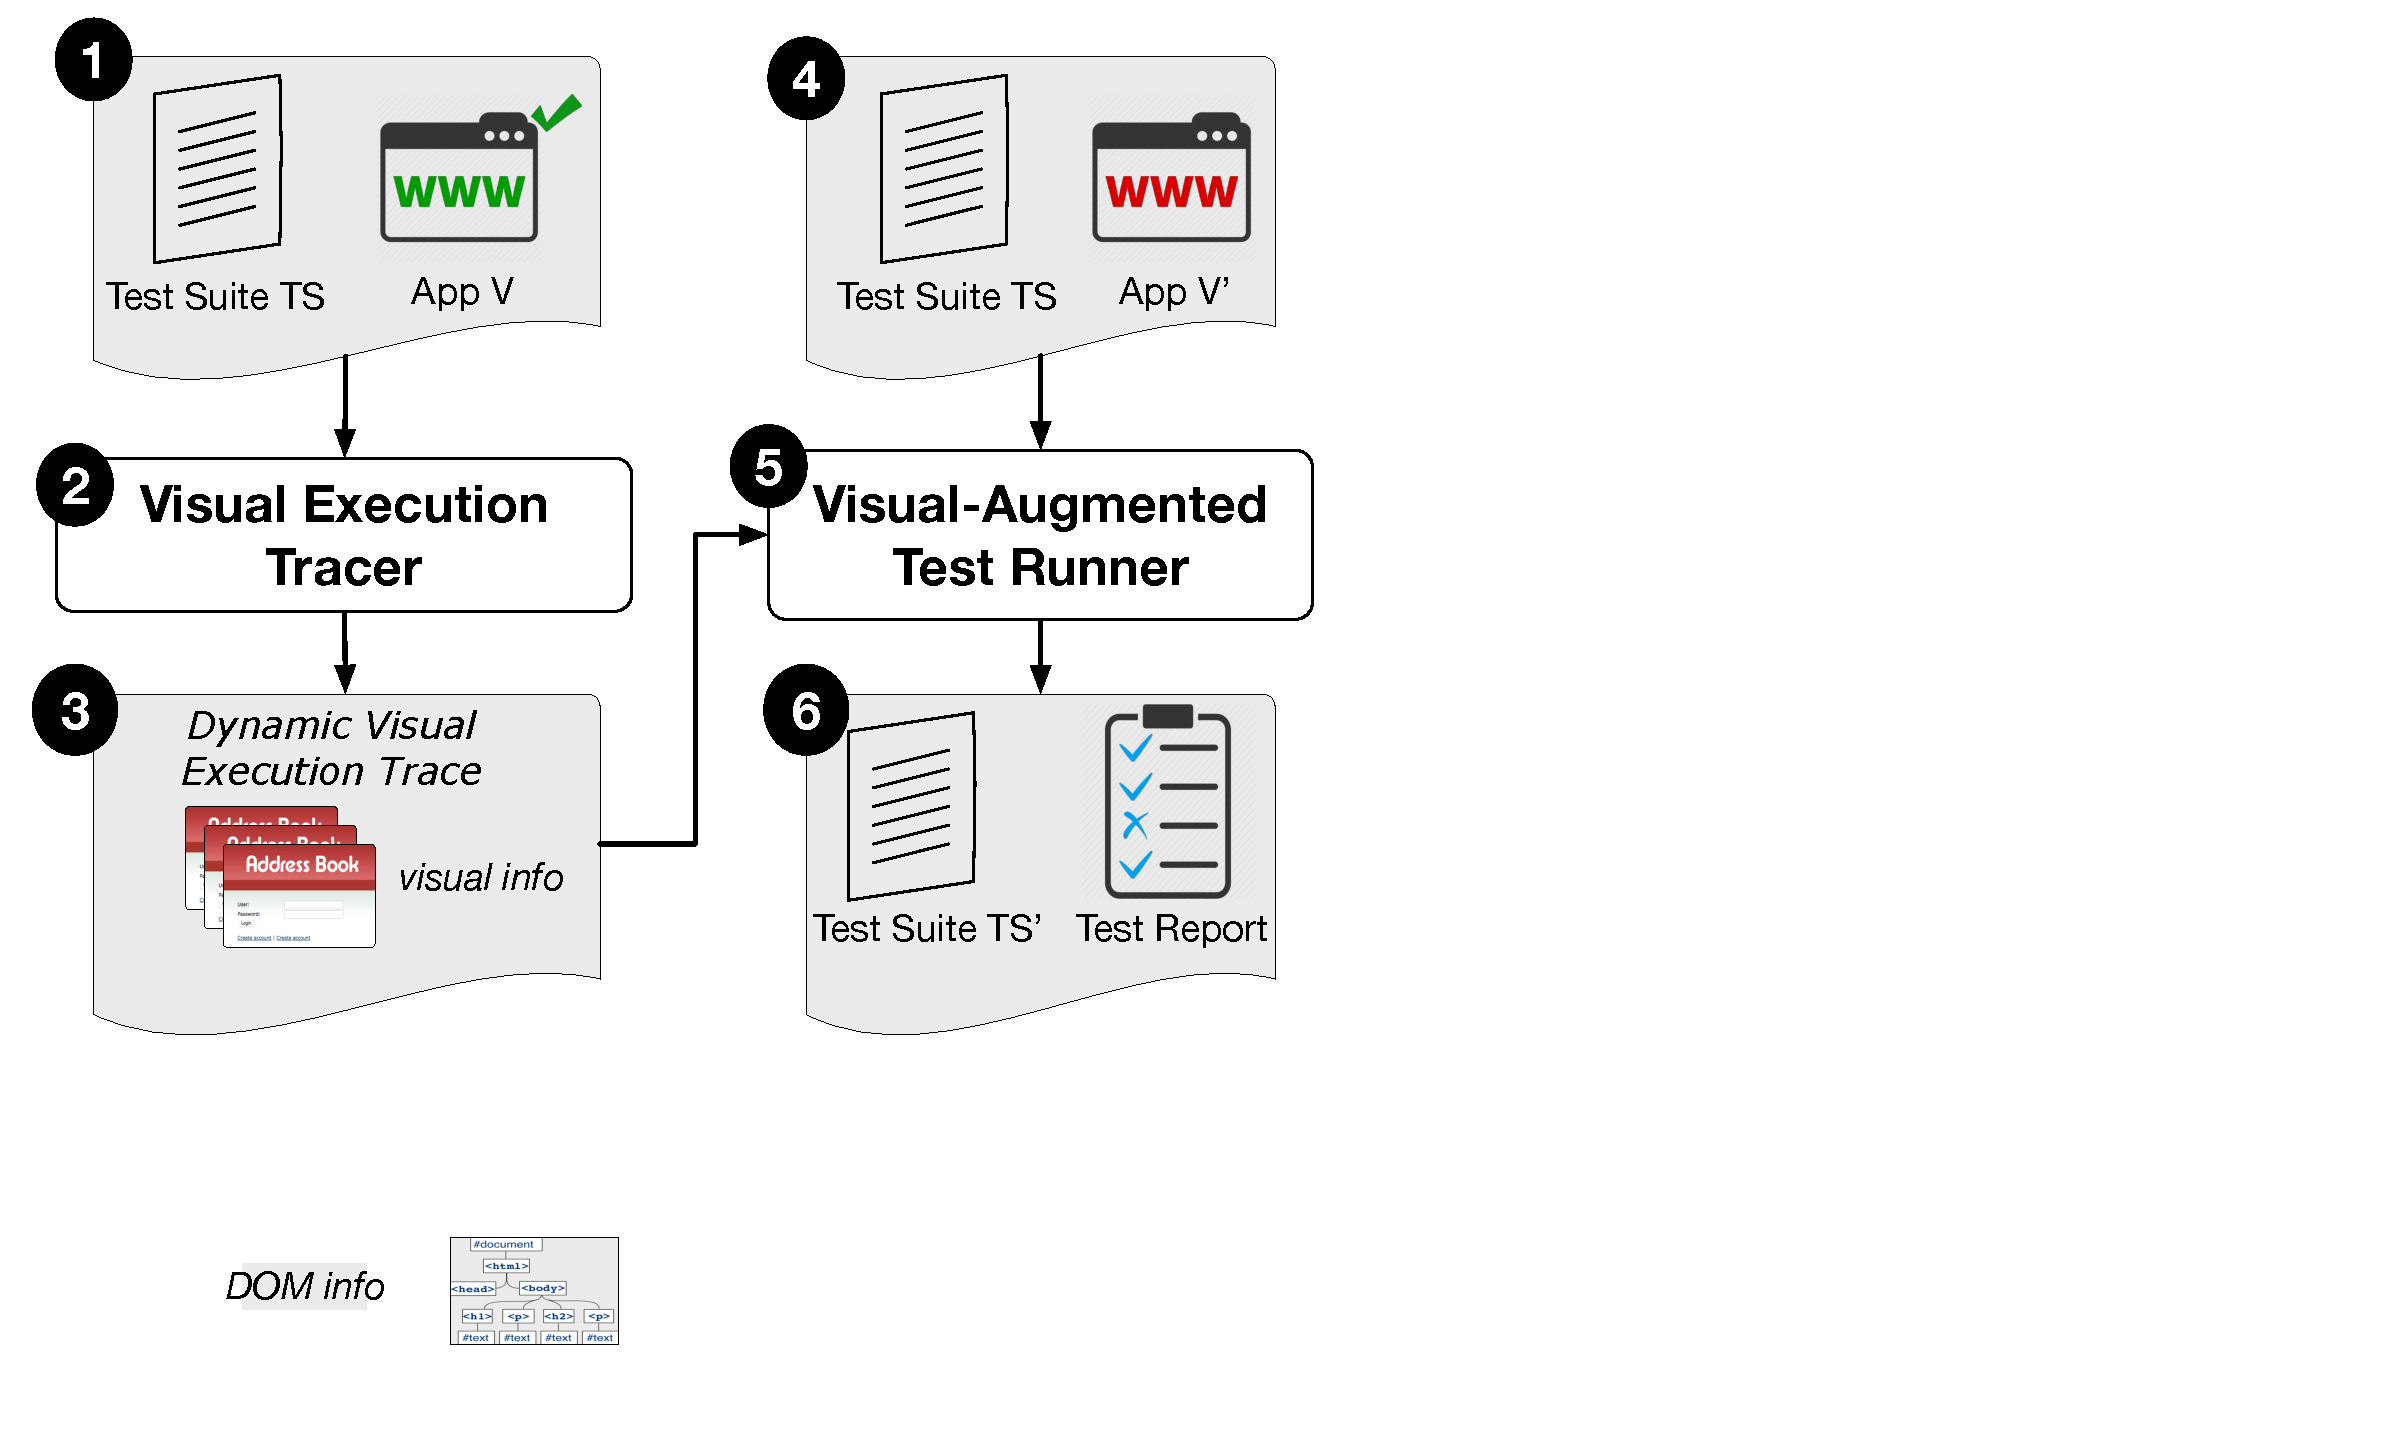
\includegraphics[trim={0.2cm 6.5cm 17cm 0.2cm},clip,scale=0.28]{images/approach-bigger}
%}
\caption{Overview of our approach. Inputs and outputs are shown as parallelograms, whereas the proposed approach is represented as rounded rectangles.}
\label{approach}
\end{figure}

\autoref{approach} illustrates the usage scenario for our approach in a real-world testing environment. 
First, given a stable version of the web application $V$ along with its working test suite $T$ (i.e., in which all test pass)~\ding{182}, a tester would run $T$ by means of the first module of \tool~\ding{183}. Such a module collects, for each test, a number of information (e.g., screenshots, DOMs)~\ding{184}. 
Then, when the application $V$ gets modified/evolved, a new version $V'$ is produced~\ding{185}. At this point, a tester may wish to use $T$ to check if regressions have occurred. To this aim, she uses the second module of \tool~\ding{186} which runs each test case of the the test suite $T$ against the new version $V'$, and makes use of the information about the previous execution traces to verify the correctness of each test statement, and eventually attempt to repair locator breakages at runtime in an \textit{online mode}. At the end of the process, \tool outputs the new verified (and eventually repaired) test suite $T'$ that works on $V'$, together with report information. 
The developer can hence manually analyse the report to decide on the correctness of the test cases. The manual effort required is potentially significantly reduced in comparison to a user carefully verifying each executing test and manually searching for fixes as breakages occur. If any of such issues exist, then the process outputs a set of repaired tests, that the developer can inspect and accept or fix manually before moving on. When the developer decides that the tests represent the intended behaviour, then $T$ can be updated to $T'$, as any subsequent app changes shall be tested against the most recent version of the test suite.
%
We now detail each step of our approach.

\subsection{Execution Trace Collection}
%
In the first phase, we need to store the DOM and visual information related to each single statement composing a test case, so as to model the runtime execution of the tests. While most of the DOM information could be collected statically, the visual appearance of the rendered elements may change during the application execution and some elements may be not visible until specific events occur. For this reason, we need to capture the visual information at runtime, while the test suite is executing. 

To this aim, the first module of \tool takes as input a web application along with its accompanying test suite, and runs each test case to collect both DOM and visual information associated to each test statement, hence creating a test model. The test model comprises a set of test states, in which both DOM and visual information are associated to each test statement. The output of this phase is a model of the runtime execution of the test suite $T$ on $V$, which we call \textit{execution trace}. %\andrea{I haven't detailed this part by means of an algorithm as references are provided}

We used and adapted the publicly available version of \textsc{PESTO}~\cite{2014-Stocco-SCAM}, a tool that uses aspect-oriented programming~\cite{aop} -- specifically the AspectJ language~\cite{aspectj} -- to intercept all Selenium WebDriver method calls (e.g., \texttt{click()}, \texttt{sendKeys()}, etc) using properly defined join-points. When a given join-point matches, advice methods store the test state \textit{before} and \textit{after} the statement's execution. The test state encompasses the following DOM-related information: \textit{(d1)}~the complete HTML page, \textit{(d2)}~the DOM, \textit{(d3)}~the XPath of the web element the test statement interacted with and \textit{(d4)}~all its HTML attributes. The collected visual information concern: \textit{(v1)}~the screenshots, \textit{(v2)}~the coordinates and size of the web element's bounding box, and \textit{(v3)}~a visual locator for it. A visual locator is the portion of the rendered web page that uniquely identifies such web element on the screen. (Note that, as explained in~\cite{2014-Stocco-SCAM,2015-Leotta-SAC}, a visual locator is not always the precise crop of the web element's bounding box. There are cases in which a larger crop -- taking into account the web element's visual context --  is necessary in order to visually differentiate it from other visually similar web elements appearing on the page, as the case of a list of input text fields in a form).

\subsection{Visual-Augmented Test Suite Runner}

\autoref{algo:alg1} illustrates the overall algorithm.

\textit{Phase 1 -- Initialization.} 
The initial part (Line~1) involves obtaining the previously saved trace execution information of the test $T$ on the reference version $V$ of the web application. 
At last, the web application $V'$ is loaded by means of Selenium WebDriver (Line~2). 

\textit{Phase 2 -- Visual-Augmented Execution.}
Such information is used to ``visually'' validate each statement $st_i$ of $T$, when executed on $V'$ (main loop Lines~4--36). The validation proceeds as follows. First, the DOM-based locator utilized by the test statement is extracted from $st_i$, along with the visual locator (e.g., an image) and the DOM information associated to the trace of $st_i$ in $V$  (Lines~5--7). Then, the \texttt{driver} instance is used to query the DOM of $V'$ to observe if the locator returns a web element (Line~8). 

\textit{Phase 3 -- Detecting and Repairing non-selection problems.}
If no elements are returned, a non-selection will occur, resulting in $st_i$ breaking in $V'$. Yet, that statement cannot be executed as-is on that test state, thus a series of countermeasures are triggered. The first heuristic tries to search for the web element visually on the same state. The \texttt{visualSearch} function (Line~11) uses advanced computer vision algorithms to match the visual representation of the web element (i.e., the visual locator captured on $V$) on the currently visualised screenshot of $V'$. The DOM information are also used to guide the search, and filter out potential outliers or visual false positives (such as visual duplicates). If a result is found, the locator of $st_i$ is updated, and the corrected statement saved in the list of repairs (Line~21--22). Then, $st_i$ is executed, and saved it as a statement of the new test case $T'$ (Lines~34--35), before to proceed to the next statement.

Conversely, even if the visual search on the same test state has failed, \tool tries a second countermeasure, by searching for the desired web element in one of the neighbouring test states of $st_i$.  Therefore, if the crawler finds a match, a new statement to reach that state (i.e, page) is created, with the corresponding web element locator, and a default ``click'' action, and added before $st_i$ in the verified list (Lines~17--18). (We currently do not support the creation of general purpose statements, such as the ones that need input data).
On the contrary, if the crawler was not able to find a match, the web element could have been removed from the web application $V'$. Thus, \tool assumes the web element as deleted, and $st_i$ is removed from the verified list (Line~15). In this case, the function \textsc{executeStatement} will not produce any action on $V'$, as well as no statements will be added to $T'$ (Lines~34--35).

\textit{Phase 4 -- Detecting and Repairing mis-selection problems.}
If a web element was returned by the initial DOM-based locator, \tool uses the DOM and visual information contained in the trace to verify whether it is still the same web element on which the test interacted with in $V$ (Lines~25--34). Additionally, in case of assertions, if the GUI textual information of the web element has changed, a new statement with the potentially corrected assertion is created and saved in the verified list (Lines~29--33). Note that, no modification are triggered to $st_i$ itself, as only the tester at a manual inspection, can verify whether the new GUI value reflects the correct behaviour of the application. Thus, the execution of $st_i$ will likely raise an \texttt{AssertionError} for the tester to inspect, for which a candidate repair has been automatically created.

\textit{Phase 5 -- Possible Outputs.}
If \autoref{algo:alg1} terminates, \tool was able to verify/correct all the statements of $T$ in the new version $V'$. If $T = T'$, no corrections have clearly been made to the test, otherwise the list of verified/corrected statements are shown to the user.
If \autoref{algo:alg1} stops prematurely, then one of the statements executed by the function \textsc{executeStatement} triggered an action that could not be performed or an incorrect locator was retrieved. The user must then intervene to manually correct such unfortunate cases.

\begin{algorithm}[b]
\scriptsize
\DontPrintSemicolon % Some LaTeX compilers require you to use \dontprintsemicolon instead
\KwIn{$T$: A test case developed for web application $V$, the URL $U$ of its subsequent version $V'$, $EX$: Execution Trace of $T$ when executed on $V$}
\KwOut{$T'$: A verified/repaired $T$ working on $V'$}
%\colorbox{lightgray}{/* Execution Trace collection */} \;
\textit{trace} $\gets$ loadExecutionTrace($EX$) \;
\textit{driver} $\gets$ loadApp($U$) \;
\textit{statements}, \textit{repairedStatements} $\gets$ getStatements(T) \;
 \ForEach{ test statement $st_i \in$ \textit{statements} }{%
  \textit{locator} $\gets$ getLocator($st_i$)\;
  \textit{\textit{visLocator}} $\gets$ getVisualLocator(\textit{trace}, $st_i$) \;
 \textit{\textit{DOMInfo}} $\gets$ getDOMInfo(\textit{trace}, $st_i$) \;
  \textit{webElement} $\gets$ \textit{driver}.findElement(\textit{locator})\;
  \HiLi{/* Manage non-selection of web element. */} \;
   \uIf{webElement == null} { 
     \textit{webElemVisual} $\gets$ \textsc{visualSearch}(\textit{driver}, $st_i$, \textit{visLocator}, \textit{DOMInfo})\;
     \uIf{\textit{webElemVisual} == null} {
       \textit{webElemVisual} $\gets$ \textsc{localCrawling}(\textit{driver}, $st_i$, \textit{visLocator}, \textit{DOMInfo})\;
       \uIf{\textit{webElemVisual} == null} {
       \textit{repairedStatements}.remove($st_i$)\;
       } \Else{
       \textit{newStmt} $\gets$ <\textsc{synthetizeLocator}(\textit{webElemVisual}), ``click'', ``''> \;
       \textit{repairedStatements}.addBefore($st_i$, \textit{newStmt}) \;
        }
     } \Else{
     updateLocator($st_i$, \textit{webElemVisual}) \;
      \textit{repairedStatements}.update($st_i$) \;
     }
   \HiLi{/* Manage mis-selection of web element. */} \;
   } \ElseIf{webElement $\neq$ null}{
      \textit{webElemVisual} $\gets$ \textsc{visualSearch}(\textit{driver}, $st_i$, \textit{visLocator}, \textit{DOMInfo})\;
     \textit{webElement} $\gets$ \textsc{verify}(\textit{webElement}, \textit{webElemVisual})\;
      \textit{repairedStatements}.update($st_i$, \textit{webElement}) \;
   }
   \HiLi{/* Suggest potential fix to assertions value. */} \;
    \If { webElement.getText() $\neq$ getTextualContent($st_i$) } {
         \textit{newStmt} $\gets$ <\textit{webElement}, ``getText'', webElement.getText()> \;
      	\textit{repairedStatements}.replace($st_i$,  \textit{newStmt}) \;
      }
         \textit{driver} $\gets$ \textsc{executeStatement}($st_i$, $V'$) \;
      	$T'$.add($st_i$) \;
 }
\Return{$T'$, \textit{repairedStatements}}\;
\caption{Overall Algorithm}
\label{algo:alg1}
\end{algorithm}

\subsection{Visual Search}

\subsection{Crawling Search}

Manually repairing every broken workflow is tedious and frustrating, since even a medium-size web application may contain tens of GUI screens and hundreds of GUI actions. It is hence likely infeasible for a tester to quickly explore this space to choose replacement actions from.

Fortunately, a web crawler can do this automatically. To this aim, \tool integrates \textsc{Crawljax}, a state of the art tool for the automatic crawling of dynamic web applications~\cite{mesbah:tweb12,mesbah:tse12}. We developed a plugin for Crawljax that incorporates the \texttt{visualSearch} function (Line~11), so that the crawler can effectively explore the state space of $V'$ looking for a visual match in all the neighbouring states of the current test state (Line~13). As a conservative choice, since the number of DOM states and events can be numerous, we set the crawling depth to one (1). On the one hand, this limits the search capability, potentially missing states in which the elements could be found. On the other hand, this choice keeps the running time acceptable.

\subsection{Implementation}\label{sec:implementation}

We implemented our approach in a tool called \tool, which is publicly available (URL omitted). 
The tool is written in Java, and supports Selenium test suites written in Java. However, our overall approach is more general and applicable to test suites developed using other programming languages or testing frameworks. 
\tool gets as input the path to the test suites, collects the visual execution traces by means of an AspectJ module, and runs the visual-augmented repair algorithms. 
\tool makes use of the traces to generate potential repairs and generates a list of repaired test cases.







